
\documentclass{jtetiproposalskripsi}

%-----------------------------------------------------------------
%Disini awal masukan untuk data proposal skripsi
%-----------------------------------------------------------------
\titleind{SISTEM PEMBELAJARAN MELALUI MEDIA ON-LINE 
(E-LEARNING) di UNIVERSITAS MUHAMMADIYAH JEMBER
}
\fullname{NUR LAILY KARTININGSIH}

\idnum{1200631014}

\approvaldate{14 Januari 2015}

\degree{Sarjana Komputer}

\yearsubmit{2015}

\program{Manajemen Informatika}

\headprogram{Sarjiya, S.T., M.T., Ph.D.}

\dept{Manajemen Informatika dan Teknik Informatika}

\firstsupervisor{Victor Wahanggara, S.Kom}
\firstnip{1203716}

\secondsupervisor{Mudafiq Ryan Pratama, S.Si}
\secondnip{1977 0131 2002 12 1 003}


%-----------------------------------------------------------------
%Disini akhir masukan untuk data proposal skripsi
%-----------------------------------------------------------------

\begin{document}

\cover

\approvalpage

%-----------------------------------------------------------------
%Disini akhir masukan untuk muka skripsi
%-----------------------------------------------------------------

%-----------------------------------------------------------------
%Disini awal masukan Intisari
%-----------------------------------------------------------------
\begin{abstractind}
Perkembangan teknologi informasi berkembang pesat, sehingga memudahkan para pengguna untuk melakukan pekerjaannya. Pada Kantor kecamatan sempu, penginputan data dan pencarian data dilakukan secara manual. Begitu juga dengan pembuatan surat permohonan yang membutuhkan waktu lama karena membuat ulang dari awal.  Dengan adanya Aplikasi surat ini dapat mengurangi ketidak akuratan penginputan data, pencarian data dan membuat surat sehingga meminimalisir waktu kerja.  Aplikasi ini juga memudahkan untuk penyimpanan berkas surat. Karena dalam aplikasi ini, setelah membuat surat permohonan terdapat pilihan untuk menyimpan surat yang telah dibuat. Sehingga mengurangi ruang penyimpanan berkas surat seperti penyimpanan berkas secara manual.  Sistem aplikasi manajemen surat ini dibuat dengan menggunakan tools seperti PHPMyAdmin dan MySQL sebagai database. Hasil dari penelitian ini adalah Sistem Aplikasi Manajemen Surat pada Kantor Kecamatan Sempu, dan dapat disimpulkan bahwa dalam perancangan aplikasi ini memberikan banyak kemudahan dalam proses pengelolaan surat. 

\bigskip
\textbf{Kata kunci} : \emph{Sistem Aplikasi Manajemen Surat, PHPMyAdmin , MySQL}.
\end{abstractind}
%-----------------------------------------------------------------
%Disini akhir masukan Intisari
%-----------------------------------------------------------------

\tableofcontents
\addcontentsline{toc}{chapter}{DAFTAR ISI}
\selectlanguage{bahasa}\clearpage\pagenumbering{arabic}\setcounter{page}{1}

%-----------------------------------------------------------------
%Disini awal masukan untuk Bab
%-----------------------------------------------------------------
\chapter{LATAR BELAKANG}

\section{Latar Belakang Masalah}
Perkembangan teknologi informasi dan komunikasi pada saat ini sudah mengalami kemajuan yang sangat pesat. Media elektronik merupakan salah satu media yang diandalkan untuk mendapatkan informasi dan merupakan komunikasi. Internet adalah jaringan komputer global yang memanfaatkan salah satu media elektronik tercanggih (komputer) untuk memenuhi segala kebutuhan informasi dan komunikasi di segala bidang dengan akses yang cepat keseluruh dunia dengan biaya relative murah.

Dengan memanfaatkan teknologi internet tersebut yang dapat diakses dalam jarak jauh dan waktu yang sangat cepat serta biaya yang relative murah, maka dunia pendidikan khususnya di Universitas Muhammadiyah Jember mulai menciptakan wahana baru dalam proses pembelajaran yaitu pembelajaran jarak jauh yang biasa di sebut dengan e-learning (elektronik  learning). Bagi institusi pendidikan, teknologi di dalam e-learning dapat dijadikan media untuk semakin memperbaiki kualitas dalam pembelajaran jarak jauh (distance learning). Banyak yang menganggap bahwa e-learning terkesan sebagai pembelajaran yang pasif dan hanya satu arah dari staf pengajar semata, sedikit demi sedikit hal ini mulai terpecahkan. Dukungan multimedia yang semakin canggih dan perkembangan baru di dunia web semakin membantu mewujudkan pembelajaran interaktif, meskipun tidak harus bertemu langsung secara fisik.

Lembaga pendidikan dimanapun sangat memerlukan e-learning sebagai wahana  pembelajaran jarak jauh yang mudah diakses. Hal tersebut dapat kita manfaatkan dengan fasilitas internet dengan mempunyai website untuk menyediakan layanan akses kepada para mahasiswa dan komponen kampus yang membutuhkan informasi terkini sehingga lebih efektif dan efisien.
Untuk mengimbangi kemajuan teknologi informasi di era globalisasi dengan memberikan konsep yang berbeda dalam proses pembelajaran yang interaktif antara mahasiswa dengan dosennya. System pembelajaran melalui media on-line (e-learning) di Universitas Muhammadiyah Jember yang sekali dibahas secara mendetail yang disertai dengan pembahasan dan aplikasinya dengan menggunakan program Macromedia Dreamweaver dan AppServer.


\section{Perumusan Masalah}
Berdasarkan uraian latar belakang diatas, maka perumusan masalah dalam laporan ini adalah :	 
\begin{itemize}
\item[1.] Bagaimana suatu Sistem Aplikasi Manajemen Surat ini dapat membantu proses register surat dan pembuatan surat di Kantor Kecamatan Sempu yang dulunya masih manual menjadi terkomputerisasi ?
\item[2.] Bagaimana membangun Sistem Aplikasi Manajemen Surat di Kantor Kecamatan Sempu Kabupaten Banyuwangi ?
\end{itemize}

\section{Batasan Masalah}

Berdasarkan uraian latar belakang diatas, maka batasan masalahnya yaitu:
\begin{itemize}
\item[1.] Khusus Sistem Aplikasi Manajemen Surat di Kantor Kecamatan Sempu Kabupaten Banyuwangi.
\item[2.] Khusus pada register data surat dinas, data surat pengajuan dan pembuatan surat dinas pada Kantor Kecamatan Sempu Banyuwangi.
\end{itemize}

\section{Tujuan Penelitian}
Adapun tujuan dari tugas akhir ini adalah merancang aplikasi kesekretariatan pada BEM Fakultas Teknik sebagai berikut :
\begin{itemize}
\item[1.] Membuat sebuah Sistem Aplikasi Manajemen Surat di Kecamatan Sempu Kabupaten Banyuwangi.
\item[2.] Membuat pengelolaan data register surat  dan pembuatan surat dinas menggunakan PHP dan MySQL sehingga laporan yang dihasilkan dan pengolahan data dapat terintegrasi dengan baik.
\end{itemize}


\section{Manfaat Penelitian}
Manfaat dari dibuatnya sistem ini yaitu :
\begin{itemize}
\item[1.] Dapat mempermudah petugas dalam memasukkan data surat ataupun pencarian data surat dan pembuatan surat dinas.
\item[2.] Meminimalisir waktu dalam pencarian data surat dan pembuatan surat.
\item[3.] Dapat mempermudah puetugas dalam mengolah surat di Kecamatan Sempu Kabupaten Banyuwangi.
\end{itemize}

%-------------------------------------------------------------------------------
\chapter{LANDASAN TEORI}               
\section{Landasan Teori}
\subsection{Sistem Informasi Manajemen }
Sistem Informasi Manajemen adalah sistem perensanaan bagian bagian dari pengendalian internal suatu bisnis yang meliputi pemanfaatan manusia, dokumen, teknologi, dan prosedur oleh akuntansi manajemen untuk memecahkan masalah bisnis. Sistem informasi manajemen dibedakan dengan sistem informasi biasa karena SIM digunakan untuk menganalisis sistem informasi lain yang diterapkan pada aktivitas operasional organisasi. Secara akademis, istilah ini umumnya digunakan untuk merujuk pada kelompok metode manajemen informasi yang bertalian dengan otomasi atau dukungan terhadap pengambilan keputusan manusia, misalnya sistem pendukung keputusan, sistem pakar, dan sistem informasi eksekutif. Sistem Informasi Manajemen merupakan sistem yang menghasilkan hasil keluaran (output) dengan menggunakan masukan (input) dan berbagai proses yang diperlukan untuk memenuhi tujuan tertentu dalam suatu kegiatan manajemen.

Menurut Kertahadi (1995) : Sistem Informasi Manajemen (SIM) dapat didefinisikan sebagai suatu alat untuk menyajikan informasi dengan cara sedemikian rupa sehingga bermanfaat bagi penerimanya...
	
Menurut Murdick dan Ross  (1993) : Tujuan sistem informasi manajemen adalah untuk menyajikan informasi guna pengambilan keputusan pada perencanaan, pemrakarsaan, pengorganisasian, pengendalian kegiatan operasi subsistem suatu perusahaan dan menyajikan sinergi organisasi pada proses.

\subsection{Sistem}
Sistem adalah sekumpulan unsur / elemen yang saling berkaitan dan saling mempengaruhi dalam melakukan kegiatan bersama untuk mencapai suatu tujuan. Jadi, secara umum Pengertian Sistem adalah perangkat unsur yang teratur saling berkaitan sehingga membentuk suatu totalitas.

Menurut R. Soemita Adikusumah dalam bukunya Sistem Prosedure dan Metode Suatu Pembahasan, Sistem adalah : “Suatu jaringan sejumlah prosedure yang saling berhubungan yang dikembangkan sesuai dengan suatu pola (rencana) untuk melakukan aktivitas utama perusahaan.”

Menurut Jogianto dalam bukunya Analisis dan Desain Sistem Informasi. Pendekatan Terstruktur Teori dan Praktek Aplikasi Bisnis bahwa sistem adalah : “Kumpulan dari elemen-elemen yang berinteraksi untuk mencapai suatu tujuan tertentu. sistem ini menggambarkan suatu kejadian-kejadian dan kesatuan yang nyata adalah suatu objek nyata, seperti tempat, benda, dan orang-orang yang betul-betul ada dan terjadi.”


\subsection{Sistem Informasi}
Sistem informasi memiliki definisi yang berbeda menurut para ahli, namun secara umum, sistem informasi adalah kombinasi dari teknologi informasi dan aktivitas orang yang menggunakan teknologi itu untuk mendukung operasi dan manajemen. Istilah ini digunakan untuk merujuk tidak hanya pada penggunaan organisasi Teknologi Informasi dan Komunikasi (TIK), tetapi juga untuk cara di mana orang berinteraksi dengan teknologi ini dalam mendukung proses bisnis.

Sementara ada juga definisi lain yang mengatakan kalau sistem informasi adalah kumpulan informasi di dalam sebuah basis data menggunakan model dan media teknologi informasi digunakan di dalam pengambilan keputusan bisnis sebuah organisasi. Di dalam suatu organisasi, informasi merupakan sesuatu yang penting di dalam mendukung proses pengambilan keputusan oleh pihak manajemen. Sistem ini memanfaatkan perangkat keras dan perangkat lunak komputer.

\subsection{Website}
Website merupakan kumpulan halaman web yang saling terhubung dan file-filenya  saling terkait. Web terdiri dari page atau halaman, dan kumpulan halaman yang dinamanakan homepage. Homepage berada dibawahnya. Biasanya setiap halaman di bawah homepage disebut child page, yang berisi hyperlink ke halaman lain dalam web.

Website awalnya merupakan suatu layanan sajian informasi yang menggunakan konsep hyperlink, yang memudahkan surfer atau pengguna internet melakukan penelusuran informasi di internet. Informasi yang disajikan dengan web menggunakan konsep multimedia, informasi dapat disajikan dengan menggunakan banyak media, seperti teks, gambar, animasi, suara atau film.

Ada beberapa kelebihan dan manfaat website sehingga banyak orang membutuhkan kehadirannya, diantaranya:
\begin{itemize}
\item •	Memiliki alamat secara online
\item •	Jangakauan tanpa batas sehingga dapat diakses oleh pengguna di seluruh dunia daam waktu yang tak terbatas.
\item •	Menjadi cermin pribadi maupun citra perusahaan apabila fitur yang disediakan cukup interaktif dan dinamis. 
\item •	Dapat berfungsi sebagai identitas pribadi / Perusahaan tentang profil diri agar dapat diketahui oleh para customer dalam menjalankan bisnis sehingga komunikasi dapat berjalan dengan mulus.
\item •	Situs personal dapat berfungsi sebagai juru bicara untuk menuangkan ide, gagasan, kritik, saran, berbagi ilmu, dan suara hati lainnya yang ingin dituangkan kedalam situs melalui tulisan.
\item •	Website yang dibuat oleh seorang pengembang website harus benar-benar mencerminkan identitas suatu institusi, jangan sampai bertolak belakang antara isi dengan bentuk dan tata letak situs itu sendiri. Ada beberapa hal yang harus diperhatikan, salah satunya adalah tentang kategori situs itu sendiri. (Gregorius, 2000: 123-124)

\end{itemize}

\subsection{PHP}
PHP adalah bahasa pemrograman script yang paling banyak dipakai saat ini, PHP banyak dipakai untuk program situs web dinamis, contoh terkenal dari aplikasi PHP adalah forum (phpBB) dan MediaWiki (software di belakang Wikipedia). PHP merupakan script yang terintegrasi dengan HTML dan berada pada server ( server side HTML embedded scripting ). PHP juga dapat dilihat sebagai pilihan lain dari ASP.NET/VB.NET Microsoft, ColdFusion Macromedia, JSP/Java Sun Microsystems, dan CGI/Perl. Contoh aplikasi lain yang lebih kompleks berupa CMS yang dibangun menggunakan PHP adalah Mambo, Joomla!, Postnuke, Xaraya, dan lain-lain. (Anhar, 2010: 10-11)

\subsection{XAMPP}
XAMPP adalah perangkat lunak bebas yang mendukung banyak sistem operasi yang merupakan kompilasi dari beberapa program. Fungsinya adalah sebagai server yang berdiri sendiri (localhost), yang terdiri atas program Apache HTTP Server, MySQL database dan penerjemah bahasa yang ditulis dengan bahasa pemrograman PHP dan Perl.

Nama XAMPP merupakan singkatan dari X (empat sistem operasi apapun), Apache, MySQL, PHP dan Perl. Program ini tersedia dalam General Public License (GNU) dan bebas, merupakan web server yang mudah digunakan yang dapat melayani tampilan halaman web yang dinamis.  
XAMPP adalah kepanjangan yang masing-masing hurufnya adalah:

X   :	Program ini dapat dijalankan dibanyak sistem operasi, seperti Windows, Linux, Mac OS, danjuga Solaris.

A   :	Apache, merupakan aplikasi web server. Tugas utama Apache adalah menghasilkan halaman web yang benar kepada user berdasarkan kode PHP yang dituliskan oleh pembuat web, maka dapat saja suatu database diakses terlebih dahulu (misalnya dalam MySQL) untuk mendukung halaman web yang dihasilkan.

M   :	MySQL, merupakan aplikasi database server. Perkembangannya disebut SQL yang merupakan kepanjangan dari Structure Query Language. SQL merupakan bahasa terstruktur yang digunakan untuk mengolah database. 
MySQL dapat digunakan untuk membuat dan mengelola database besertaisinya. Kita dapat memanfaatkan MySQL untuk menambahkan, mengubah dan menghapus data yang berada dalam database.

P    :	PHP, bahasa pemrograman web. Bahasa pemrograman PHP merupakan bahasa pemrograman untuk membuat web yang bersifat server-side scripting. PHP memungkinkan kita untuk membuat halaman web yang bersifat dinamis. Sistem manajemen basis data yang sering digunakan bersama PHP adalah MySQL.

P    :	Perl adalah bahasa pemrograman untuk segala keperluan, dikembangkan pertama kali oleh Larry Wall di mesin Unix. Perl dirilis pertama kali pada tanggal 18 Desember 1987 ditandai dengan keluarnya Perl 1.

Pada versi-versi selanjutnya, Perl tersedia pula untuk berbagai sistem operasi varian Unix (SunOS, Linux, BSD, HP-UX), juga tersedia untuk sistem operasi seperti DOS, Windows, Power PC, BeOS, VMS, EBCDIC, dan PocketPC. (Rachmad Hakim, 2010: 120-121)

\subsection{MYSQL}
MySQL merupakan sebuah basis data yang mengandung satu atau beberapa kolom. Tabel terdiri atas sejumlah basis dan setiap baris mengandung satu atau beberapa kolom. Didalam PHP telah menyediakan fungsi untuk koneksi ke basis data dengan sejumlah fungsi untuk pengaturan baik menghubungkan maupun memutuskan koneksi server database MySQL sebagai sarana untuk mengumpulkan informasi. (Yeni Kustiyahningsih, Devie Rosa Anamisa, 2010: 145-146).

Database adalah sistem penyimpanan beragam jenis data dalam sebuah entitas yang besar untuk diolah sedemikian rupa agar mudah dipergunakan lagi. Data yang disimpan bisa sangat variatif (angka, teks, gambar, suara, dan jenis data multi-media lainnya). Basis data merupakan kumpulan dari data yang saling berhubungan satu dengan yang lainnya, tersimpan di perangkat keras computer dan digunakan perangkat lunak untuk memanipulasinya. Database merupakan salah satu komponen yang penting dalam sistem informasi,karena merupakan basis dalam menyediakan informasi bagi para pemakai. (Sucipto, 2012: 137).
MySQL adalah sistem manajemen basisdata relasi yang bersifat terbuka atau open source. Sistem manajemen basisdata ini adalah hasil pemikiran dari Michael “Monty” Widenius, David Axmark, dan Allan Larson pada tahun 1995. 

Tujuan awal ditulisnya program MySQL adalah untuk mengembangkan aplikasi web. MySQL menggunakan bahasa standar SQL (Structure Query Language) sebagai bahasa interaktif dalam mengelola data. 
Perintah SQL sering juga disebut Query. MySQL menawarkan berbagai keunggulan dibandingkan database server lain.


%-------------------------------------------------------------------------------
\chapter{METODE PENELITIAN}

\section{Flowchart Metode Penelitian}
\begin{figure}[h]
\centering 
 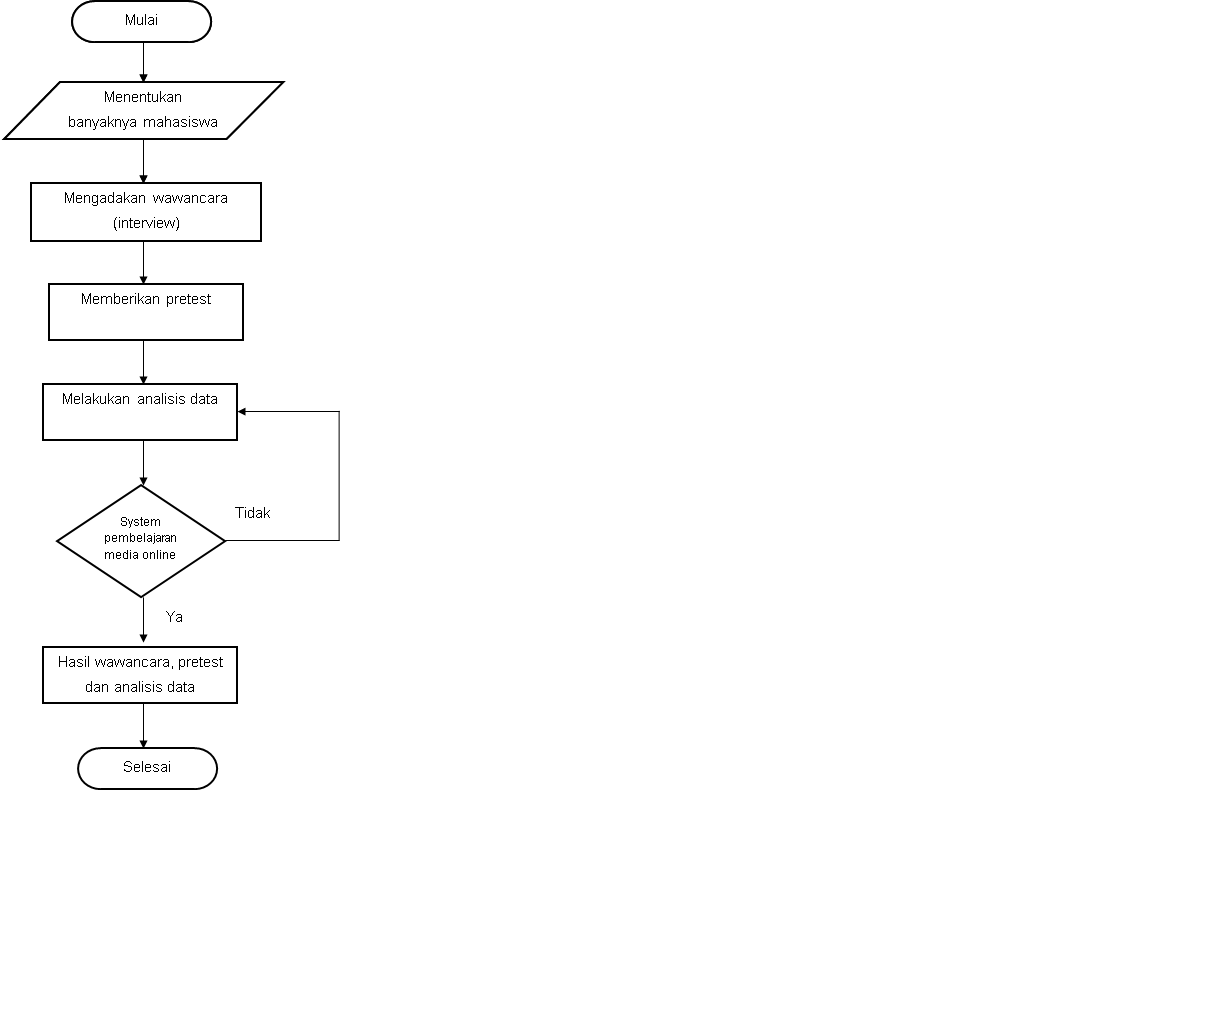
\includegraphics[width=0.7\textwidth]{gambar/1}  
 \caption{Flowchart Metode Penelitian}
\end{figure}

\section{Alat dan Bahan}
Bahan yang digunakan dalam penelitian ini adalah:

\vspace{-0.5cm}

\begin{enumerate}[a.]
\begin{singlespace}
\itemsep0em
\item Laptop/PC (2 unit),
\item Sistem Operasi (Windows 7),
\item Neatbean IDE 7.2 (Java),
\item Microsoft Visio 2010,
\item MySQL Workbench 6.0 (database),
\item Wifi/Modem (Koneksi Internet).
\end{singlespace}
\end{enumerate}

\section{Prosedur Penelitian}

Untuk dapat melaksankan tahapan penelitian maka tahapan penelitian yang dilakukan adalah sebagai berikut: 
\subsection{Studi Pustaka}

Studi pustaka dilakukan untuk mencari informasi - informasi tentang teori, metode dan konsep yang relevan dengan permasalahan. Sehingga dengan informasi – informasi tersebut dapat digunakan sebagai acuan dalam penyelesaian masalah. Studi pustaka yang dilakukan dengan mencari informasi dan referensi dalam bentuk text book, literatur, informasi dari internet maupun sumber-sumber lainnya yang berkaitan dengan penelitian ini.

\subsection{Metode Pengumpulan data}
Pengumpulan data dilakukan untuk memperoleh informasi yang dibutuhkan dalam rangka mencapai tujuan penelitian. Tujuan yang diungkapkan dalam bentuk hipotesis merupakan jawaban sementara terhadap pertanyaan penelitian.


\section{Jadwal Kegiatan}
Dalam melaksanakan tahapan penilitian agar penelitian tersebut dapat diselesaikan sesuai dengan waktu yang direncanakan maka peneliti membuat matrik berupa tahapan jadwal penelitian sebagai berikut:

\begin{center}
Tabel 3.1. Jadwal Penelitian.
\end{center}
\vspace{-0.5cm}
\begin{figure}[ht!]
  \centering
    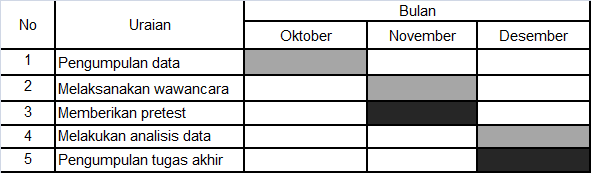
\includegraphics[width=17cm]{gambar/3}
\end{figure}

%-----------------------------------------------------------------
%Disini akhir masukan Bab
%-----------------------------------------------------------------

%-----------------------------------------------------------------
%Disini awal masukan untuk Daftar Pustaka
%-----------------------------------------------------------------
%%\nocite{Abel2010,Guerbas201350}
%%\bibliography{research-plan}
%%\bibliographystyle{plainnat}
\begin{thebibliography}{9}

\bibitem[satu(2013)]{satu01}
Anhar.Panduan Menguasai PHP dan MySQL, Jakarta, 2010

\bibitem[dua(2013)]{dua02}
Devie Rosa Anamisa. Yeni Kustiyahningsih. Pemrograman Basis Data Berbasis Web Menggunakan PHP dan MySQL, Bangkalan, 2010

\bibitem[tiga(2013)]{tiga03}
Sucipto. Konsep dan Teknik Pengembangan Sistem berbasis Teknologi Informasi : Banten, 2010

\bibitem[empat(2013)]{empat04}
Hakim. Rachmad. Cara Mengelola Blog, Elexmedia Komputindo : Jakarta, 2010

\bibitem[lima(2013)]{lima05}
Sucipto. Sistem Informasi Manajemen Berbasis Tren Teknologi Informasi : Tangerang, 2012

\bibitem[enam(2013)]{enam06}
Virgi. Cepat Mahir Pemrograman Web dengan PHP dan MySQL : Jakarta, 2011

\bibitem[tujuh(2013)]{tujuh07}
Jogiyanto. Analisis dan Desain Sistem Informasi. Pendekatan Terstruktur Teori dan Praktek Aplikasi Bisnis : Yogyakarta, Andi. 2001

\bibitem[delapan(2013)]{delapan08}
Dokumen online, www.wikipedia.com/sistem-informasi-manajemen.html, Sistem Informasi Manajemen, diakses pada November 2014

\bibitem[sembilan(2013)]{sembilan09}
Dokumen online, www.informasiharian.com/sistem-manajemen-informasi-pengertian-dan-tujuan.html, Sistem, diakses pada November 2014

\end{thebibliography}
\addcontentsline{toc}{chapter}{DAFTAR PUSTAKA}
%-----------------------------------------------------------------
%Disini akhir masukan Daftar Pustaka
%-----------------------------------------------------------------

\end{document}